\documentclass{article}
\usepackage{amsmath,amssymb,bbm,comment,graphicx,amsthm,gensymb}
\usepackage[margin=2.5cm]{geometry}
\title{Linear Decision Rule Approach}
\author{Zhan Lin}

%\renewcommand{\arraystretch}{1.5}
\linespread{1.6}
\date{}
\begin{document}
\maketitle
\section{Original Problem}
Consider a network system consisting of $m$ resources, with capacity levels $\mathbf{c}=(c_1,\ldots,c_m)^T$, and $n$ products, with corresponding prices denoted by $\mathbf{v} = (v_1,\ldots,v_n)^T$. Each products needs at most one unit of each resource. Let $A = \left(a_{ij}\right)$ be the resource coefficient matrix, where $a_{ij}=1$ if product j uses one unit of resource i and $a_{ij}=0$ otherwise. Define $\xi = \left(1, \xi_{1,1}, \xi_{1,2}, \ldots, \xi_{1,n}, \ldots, \xi_{t,1}, \xi_{t,2}, \ldots, \xi_{t,n} \right)^T $ where $\xi_{t,j}$ is demand of product $j$ in period $t$. Assuming observing $\tau$ periods of history,let $\xi^t$ be the observed history demands, $\xi_t$ be the demand at period t and $$\mathbf{x_t}(\xi^{t-1},\xi_t) = \left(x_{t,1}(\xi^{t-1},\xi_{t,1}),x_{t,2}(\xi^{t-1},\xi_{t,2}),\ldots,x_{t,n}(\xi^{t-1},\xi_{t,n})\right)^T$$ be the booking limits in period t. Realisation of $\xi$ is limited to $\Xi$. The optimality equations can be expressed as

\begin{equation}
\begin{array}{ll}
\max\limits_{\mathbf{x_t}} &\mathbb{E}_{\xi}\left(\sum\limits^T_{t=1} \mathbf{v}^T \mathbf{x_t} \left(\xi^{t-1},\xi_t\right)\right)\\
s.t. & \sum\limits^T_{t=1} A \mathbf{x_t} \left(\xi^{t-1},\xi_t\right) \leq \mathbf{c}\\
& \mathbf{x_t}(\xi^{t-1},\xi_t) \geq 0\\
&\forall \xi \in \Xi,t=1,\ldots,T
\end{array}
\label{origin}
\end{equation}

It's important to notice that actually $x_{t,j}(\xi^{t-1},\xi_t) = u(\xi^{t-1}) \bigwedge \xi_t$.If making decisions without $\xi^{t-1}$, we will have $x_{t,j}(\xi_t)=u\bigwedge \xi_t$ and equation \ref{ignoreorigin} .

\begin{equation}
\begin{array}{ll}
\max\limits_{\mathbf{x_t}} &\mathbb{E}_{\xi}\left(\sum\limits^T_{t=1} \mathbf{v}^T \mathbf{x_t} \left(\xi_t\right)\right)\\
s.t. & \sum\limits^T_{t=1} A \mathbf{x_t} \left(\xi_t\right) \leq \mathbf{c}\\
& \mathbf{x_t}(\xi_t) \geq 0\\
&\forall \xi \in \Xi,t=1,\ldots,T
\end{array}
\label{ignoreorigin}
\end{equation}

Equation \ref{ignoreorigin} can be reformulated as the following equation \ref{originsec} according to Preservation of Structural Properties in Optimization
with Decisions Truncated by Random Variables and
Its Applications.

\begin{equation}
\begin{array}{ll}
\max\limits_{\mathbf{\mathcal{X}_t}} &\mathbb{E}_{\xi}\left(\sum\limits^T_{t=1} \mathbf{v}^T \mathbf{\mathcal{X}_t}\left(\xi_t\right)\right)\\
s.t. & \mathcal{X}_t(\xi_t) \leq \xi_t\\
& \{\mathbf{\mathcal{X}_t}(\xi_t) = (\mathcal{X}_{t,1}(\xi_{t,1}),\mathcal{X}_{t,2}(\xi_{t,2})\ldots,\mathcal{X}_{t,j}(\xi_{t,j}))^T\} \in \mathcal{F}\\
&\forall \xi \in \Xi,t=1,\ldots,T
\end{array}
\label{originsec}
\end{equation}
where $\mathcal{F}=\{\{f(\xi_t)\}:f(\xi_t) = \mathbf{u}_t\bigwedge \xi_t,u_t\in\mathbb{R}^+,\sum\limits^T_{t=1} A \mathbf{u_t}\leq \mathbf{c}\}$.

\section{Linear Decision Rule Approach via Lifting}
\subsection{Piecewise Linear Continuous Decision Rules with Axial Segmentation}
Define
$$
L(\xi)=(L_{t,j}(\xi_{t,j}))_{t \times j \times r,1}
$$

where $$L_{t,j}(x) = (L_{t,j,d}(x))_{r\times1}$$
and
$$
L_{t,j,d}(x)  =
\left\{
\begin{array}{ll}
x & r = 1\\
\min\{x,z_1^{t,j}\}& r>1,d=1\\
\max\{\min\{x,z_d^{t,j}\}-z^{t,j}_{d-1},0\} & r>1,d=2,\ldots,r-1\\
\max\{x-z_{d-1}^{t,j},0\}& r>1,d=r
\end{array}
\right.
$$
as show in figure \ref{L}.

\begin{figure}
\centering
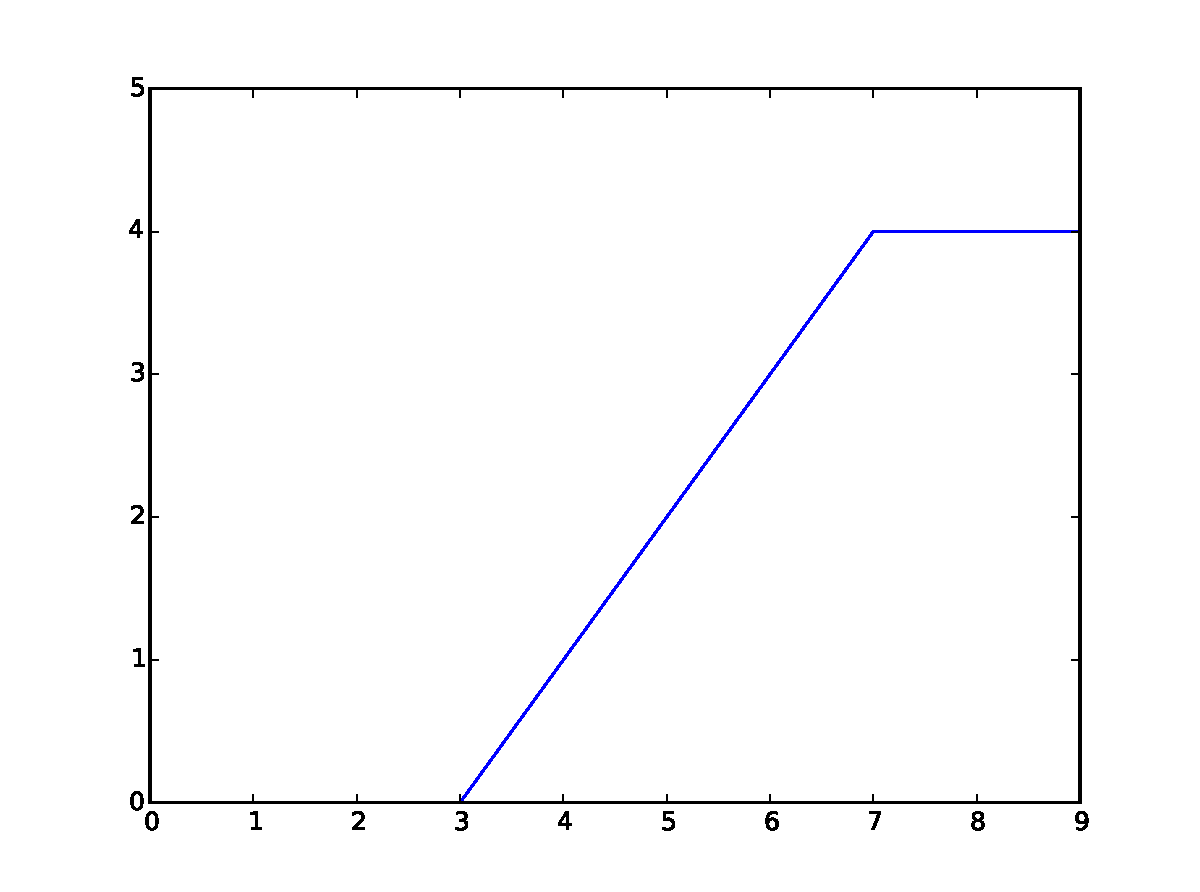
\includegraphics[width=.7\textwidth]{plf_0.pdf}
\caption{piecewise linear function}\label{L}
\end{figure}


It is obvious that the linear retraction operator corresponding to $L_{t,j}$ is $$R_{t,j}(y)=\sum\limits^{r}_{d=1} y_d=e^T y$$
\subsection{Primal Problem}
Approach equation \ref{originsec} with $$x_{t,j}(\xi_{t,j})=\tilde{X}_{t,j}Q_{t,j}L(\xi)$$ where $\tilde{X}$ and $Q_{t,j}$ are both matrixes meanwhile $Q_{t,j}$ restricts $L(\xi)$ to $L(\xi_{t,j})$.

According to \cite{GDR},
with $\Xi = \left\{ \xi : \xi_1=1,l_{t,j}\leq \xi_{t,j} \leq r_{t,j}\right\}$ and $\Xi'$ = $L(\Xi)$,
$$\text{conv}\Xi'=\left\{\xi' : \xi_1'=1,V_{t,j}^{-1}(1,\xi_{t,j}')_{(r+1)\times1}^T\geq 0\right\}$$
$$
V_{t,j}^{-1}=\begin{pmatrix}
\frac{z^{t,j}_1}{z^{t,j}_1-l_{t,j}} & -\frac{1}{z^{t,j}_1-l_{t,j}}& & & &\\
-\frac{l_{t,j}}{z^{t,j}_1-l_{t,j}}& \frac{1}{z^{t,j}_1-l_{t,j}}& -\frac{1}{z^{t,j}_2-z^{t,j}_1}& & &\\
& &\frac{1}{z^{t,j}_2-z^{t,j}_1}&\ddots & &\\
& & &\ddots& -\frac{1}{z^{t,j}_{r-1}-z^{t,j}_{r-2}}&\\
& & & &\frac{1}{z^{t,j}_{r-1}-z^{t,j}_{r-2} }&-\frac{1}{u_{t,j}-z^{t,j}_{r-1}}\\
& & & & & \frac{1}{u_{t,j}-z^{t,j}_{r-1}}
\end{pmatrix}
$$
Then we obtain the primal problem equation \ref{primal}
\begin{equation}
\begin{array}{ll}
\max\limits_{\tilde{X}_{t,k}} &\mathbb{E}_{\xi}\left(\sum\limits^T_{t=1} \mathbf{v}^T ( \sum\limits_{k=1}^j\tilde{X}_{t,k}Q_{t,k})\xi\right)\\
\text{s.t.} & \sum\limits^T_{t=1} A ( \sum\limits_{k=1}^j\tilde{X}_{t,k}Q_{t,k})\xi \leq 2\mathbf{c} - \mathbb{E}_{\xi}\left(\sum\limits^T_{t=1} A ( \sum\limits_{k=1}^j\tilde{X}_{t,k}Q_{t,k})\xi\right)\\
& \tilde{X}_{t,k}Q_{t,k}\xi \leq e^T Q_{t,k}\xi\\
& \tilde{X}_{t,k}Q_{t,k}\xi \geq 0\\
&\forall \xi \in \text{conv}\Xi' ,t=1,\ldots,T,k=1,\ldots,j
\end{array}
\label{primal}
\end{equation}

The correction $\mathbf{c} - \mathbb{E}_{\xi}\left(\sum\limits^T_{t=1} A (\sum\limits_{k=1}^j\tilde{X}_{t,k}Q_{t,k})\xi\right) $arises from inaccurately approaching $\mathbf{x}(\xi^{t-1},\xi_t)$.Also, there are $O( n^2 t^2 r )$ variables and $O(t^2 n^2 r+t n m r)$ constraints in total.

The solution $\tilde{X}_{t,j}(\xi_{t,j})$ of equation \ref{primal} has same structure with either figure \ref{plf:1} or figure \ref{plf:2}.The proof is trivial.
\begin{proof}
As we can see from constraints, defining $\tilde{X}_{t,k}(\xi_{t,k}) = \tilde{X}_{t,k}Q_{t,k}\xi$, $\tilde{X}_{t,k}(\xi_{t,k}) \leq \xi_{t,k}$. Therefore the angle at $(0,0)$ must less than $45\degree$. On the other hand, if we keep $\tilde{X}_{t,k}(\xi_{t,k})$ no longer growing after the maximum point, it will never violate constraints as it doesn't need more resource than the maximum point which could be achieved. So $\tilde{X}_{t,k}(\xi_{t,k})$ must be flatten after the break point. It also hint us that we could learn booking limits from the break point.
\end{proof}

\begin{figure}
\centering
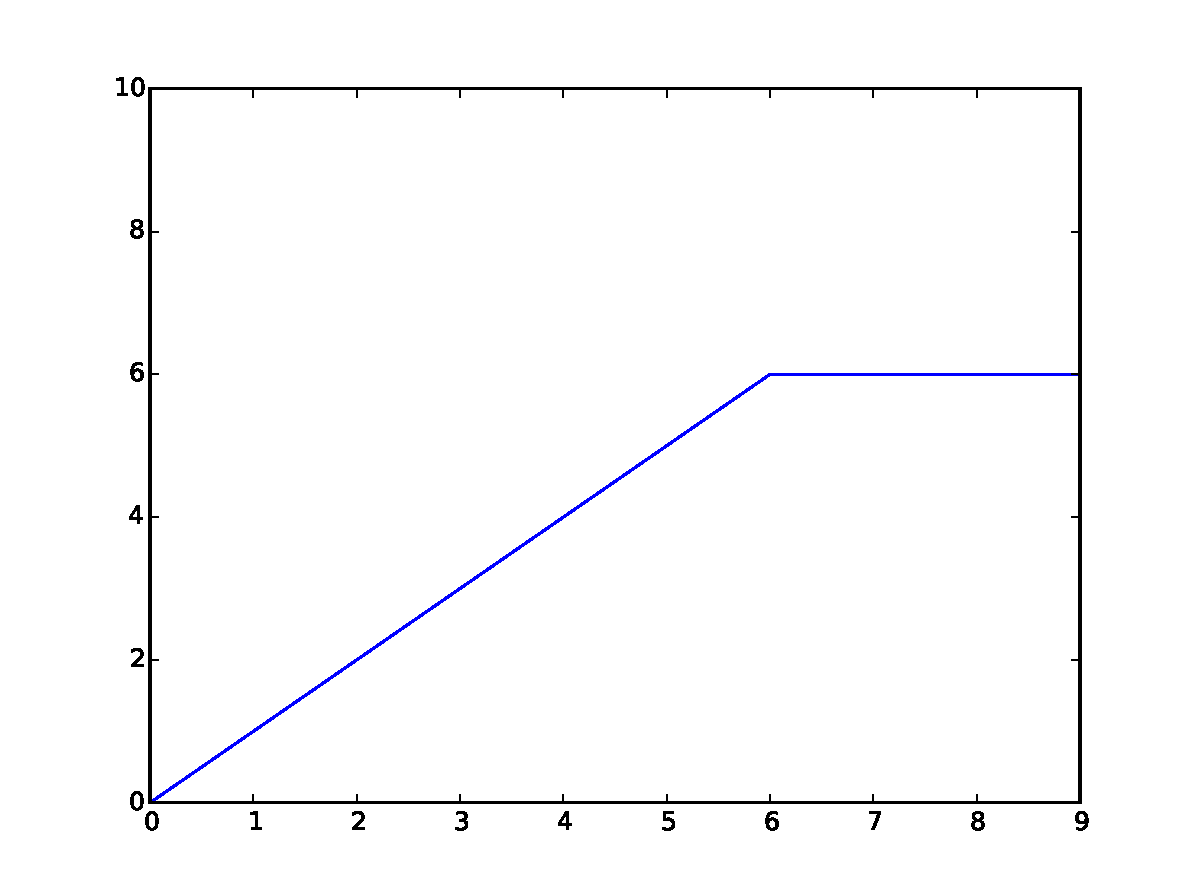
\includegraphics[width=.7\textwidth]{plf_1.pdf}
\caption{$z^{t,j}_{k}$ happened to be a break point}\label{plf:1}
\end{figure}

\begin{figure}
\centering
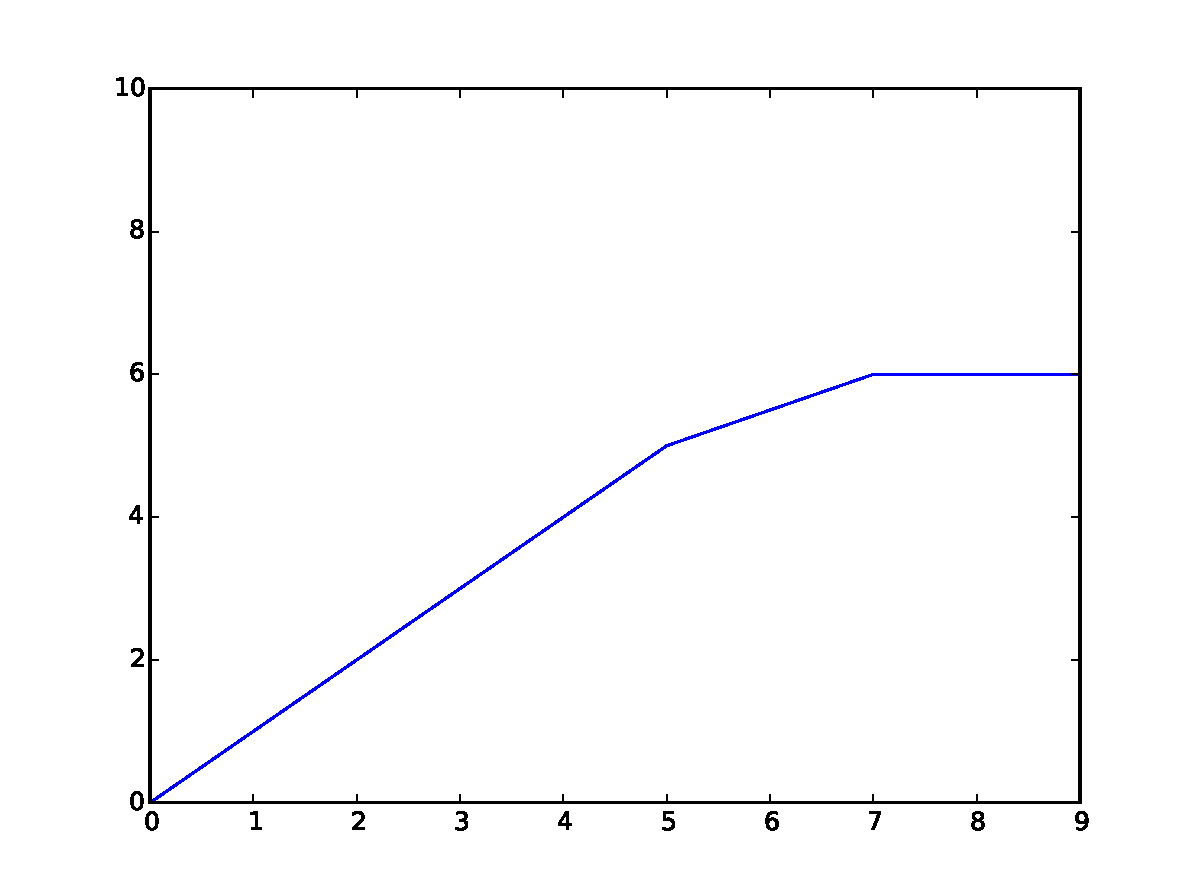
\includegraphics[width=.7\textwidth]{plf_2.pdf}
\caption{every $z^{t,j}_{k}$ could not be a break point}\label{plf:2}
\end{figure}

However, the problem is that we cannot adjust booking limits dynamically with information before the clock. Elements of $\tilde{X}_{t,j}$ are not able to do changes when information is provided. Another way to approach the process is adding items $X_t P_t L(\xi)$ as shown below. $P_t$ will restrict $L(\xi)$ to $L(\xi^{t-1})$. In that case, we need to set low bound of $\xi_{t,j}$ greater than $0$.
There will be $O(n m rt \tau + n^2 t^2 r )$ variables and $O(t^2 n^2 r+t n m r)$ constraints in total.

\begin{equation}
\begin{array}{ll}
\max\limits_{X,\tilde{X}_{t,k}} &\mathbb{E}_{\xi}\left(\sum\limits^T_{t=1} \mathbf{v}^T (X_t P_t + \sum\limits_{k=1}^j\tilde{X}_{t,k}Q_{t,k})\xi\right)\\
\text{s.t.} & \sum\limits^T_{t=1} A (X_t P_t + \sum\limits_{k=1}^j\tilde{X}_{t,k}Q_{t,k})\xi \leq 2\mathbf{c} - \mathbb{E}_{\xi}\left(\sum\limits^T_{t=1} A (X_t P_t + \sum\limits_{k=1}^j\tilde{X}_{t,k}Q_{t,k})\xi\right)\\
& (X_t P_t + \sum\limits_{k=1}^j\tilde{X}_{t,k}Q_{t,k})\xi \leq e^T Q_{t,k}\xi\\
& (X_t P_t + \sum\limits_{k=1}^j\tilde{X}_{t,k}Q_{t,k})\xi \geq 0\\
&\forall \xi \in \text{conv}\Xi' ,t=1,\ldots,T
\end{array}
\label{primalsec}
\end{equation}


\begin{figure}
\centering
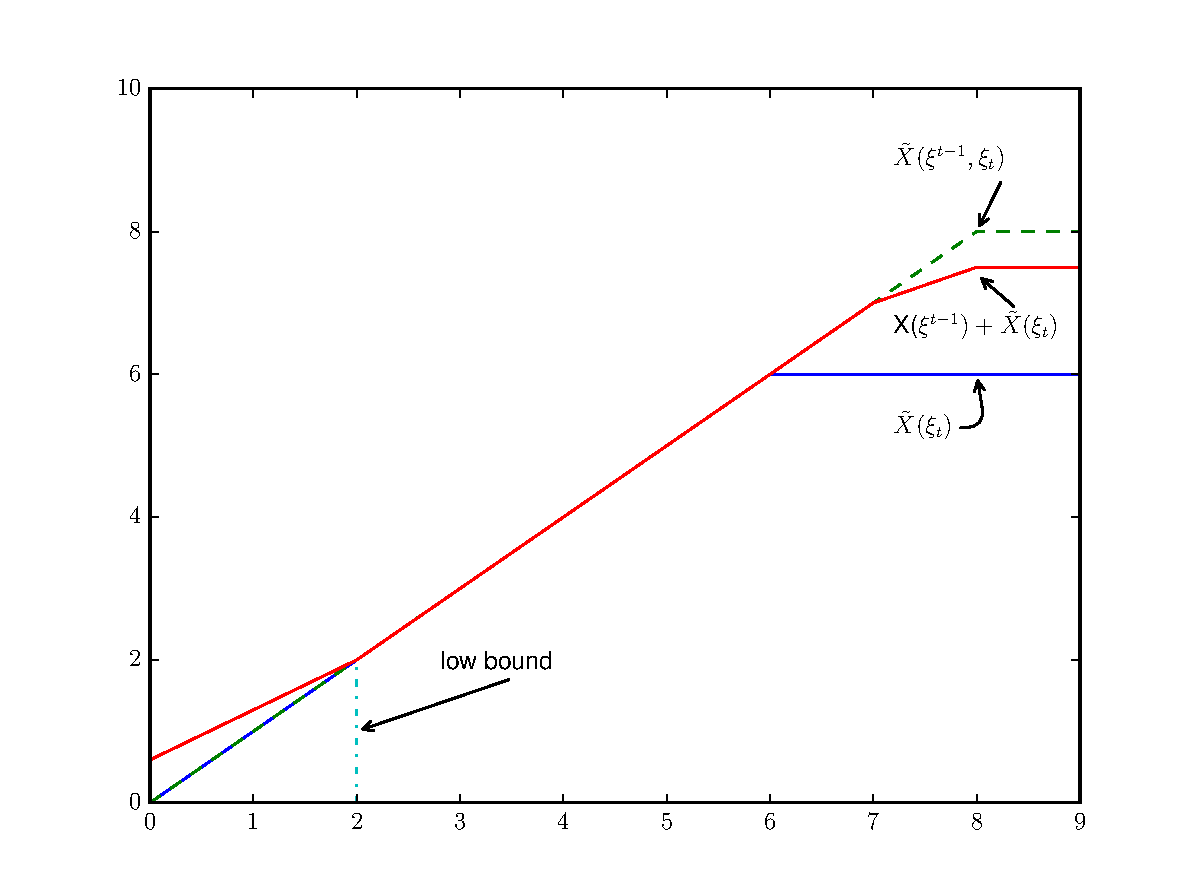
\includegraphics[width=\textwidth]{compara.pdf}
\caption{shape of functions}
\end{figure}
\begin{comment}
\subsection{Duality}

Firstly we transform equation(\ref{origin}) into a tighter formulation.
\begin{equation}
\begin{array}{ll}
\max &\mathbb{E}_{\xi}\left(\sum^T_{t=1} \mathbf{v}^T \mathbf{x_t} \left(\xi^{t-1}\right)\right)\\
s.t. & \sum^T_{t=1} \tilde{A} \mathbf{x_t} \left(\xi^{t-1}\right) \leq \mathbf{ \tilde{c}}_t\left(\xi\right)\\
& \mathbf{x_t} \left(\xi^{t-1}\right) \geq 0\\
&\forall \xi \in \Xi,t=1,\ldots,T
\end{array}
\label{duality:origin}
\end{equation}
Then it has a duality.

\begin{equation}
\begin{array}{ll}
\min &\mathbb{E}_{\xi}\left(\sum^T_{t=1}  \mathbf{ \tilde{c}}_t\left(\xi\right)^T \mathbf{y_t} \left(\xi^{t-1}\right)\right)\\
s.t. & \sum^T_{t=1} \tilde{A}^T \mathbf{y_t} \left(\xi^{t-1}\right) \geq \mathbf{v}^T\\
& \mathbf{y_t} \left(\xi^{t-1}\right) \geq 0\\
&\forall \xi \in \Xi,t=1,\ldots,T
\end{array}
\end{equation}
We can apply same approach and obtain

\begin{equation}
\begin{array}{ll}
\min &\mathbb{E}_{\xi}\left(\sum^T_{t=1}  \left(\mathbf{c}^T,(p_t\xi)^T \right)\mathbf{y_t} \left(\xi^{t-1}\right)\right)\\
s.t. & \sum^T_{t=1} \tilde{A}^T Y_t P_t \xi \geq \mathbf{v}^T\\
& Y_t P_t \xi  \geq 0\\
&\forall \xi \in \Xi\left\{ \xi : W \xi \leq h\right\},t=1,\ldots,T
\end{array}
\end{equation}
\end{comment}
\section{Computational Results}
\begin{comment}
As we can see from Preservation of Structural Properties in Optimization with Decisions Truncated by Random Variables and Its Applications,
\end{comment}
As we have shown above,
$\tilde{X}_{t,j}(\xi^{t-1},\xi_{t,j})$ should equal $u_{t,j}(\xi^{t-1})\bigwedge \xi_{t,j}$
. Benefiting from piecewise linear function, the structure is preserved with linear decision rule. Therefore, it's convenient to implement the policy as we can get $u$ from $\tilde{X}_{t,j}$. Results are computed at servers locating at USTC with 96 Intel Xeon CPU E5-4657L v2 2.4GHz and 256GB memory. Gurobi will make use of 32 cpu to solve the LP problem parallelly.
\begin{comment}
\subsection{Parameters}

The upper bound and lower bound of $\xi$ in $\Xi$ play important roles in optimizing. With strict bounds, booking limits will be under rigorous limitations. Therefore we need to set lower bound of the primal problem a bit higher. In the first example of Re-Solving Stochastic Programming Models for Airline Revenue, upper bound = 80 percentile and lower bound = 60 percentile. In the second example, upper bound = 90 percentile and lower bound = 70 percentile. Results are given at table \ref{Summary}. The results of data from approximate linear programming are not listed here. But in most cases, comparing with approximate linear programming, linear decision rules will only result in 5 percentile loss.
\end{comment}
\begin{table}[]
\centering
\begin{tabular}{|l|c|c|c|c|c|}
\hline
                                  & DLP-alloc & SLP-alloc & ceil&objective value  \\ \hline
Example 1 without re-solving  & 401980    & 415410    & 413227& 409255      \\ \hline
Example 1 with re-solving     & 409740    & 421894         & &       \\ \hline
reduction of ALP & & &18844 &18159 \\
\hline
\end{tabular}
\caption{Only depend on $\xi_t$}

\begin{tabular}{|l|c|c|c|c|}
\hline
                                 &floor(x)+1&floor(x)+2&floor(x)+3&Wait-and-see/truth value\\ \hline
Example 1 without re-solving  &417761&420294&414305&432730    \\ \hline
Example 1 with re-solving       &     &&      &432730       \\ \hline
reduction of ALP & 19414&19038 &18474 & 20411\\\hline
\end{tabular}
\caption{Only depend on $\xi_t$}
\label{Summary}
\end{table}

\begin{table}[]
\centering
\begin{tabular}{|l|c|c|c|c|c|}
\hline
                                  & DLP-alloc & SLP-alloc & ceil&objective value  \\ \hline
Example 1 without re-solving  & 401980    & 415410    & 413477& 410787      \\ \hline
Example 1 with re-solving     & 409740    & 421894      & &   \\ \hline
reduction of ALP & & &18903 &18155 \\
\hline
\end{tabular}
\caption{Depend both on $\xi^{t-1}$ and $\xi_t$}

\begin{tabular}{|l|c|c|c|c|}
\hline
                                 &floor(x)+1&floor(x)+2&floor(x)+3&Wait-and-see/truth value\\ \hline
Example 1 without re-solving  &418139&420341&414183&432730    \\ \hline
Example 1 with re-solving       &     &&      &432730       \\ \hline
reduction of ALP & 19430&18893 &18425 & 20411\\\hline
\end{tabular}
\caption{Depend both on $\xi^{t-1}$ and $\xi_t$}
\label{Summary}
\end{table}
\begin{table}[]
\centering
\begin{tabular}{|l|c|c|c|}
\hline
Case&Parameters& Solving LP Time/s& Total Time/s\\
\hline
reduction of ALP(Only depend on $\xi_t)$&$t=5,\tau=0,r=10$& 6.3&86.7\\
\hline
reduction of ALP(Depend on both $\xi^{t-1}$ and $\xi_t$)&$t=5,\tau=5,r=10$& 41.07&137.83\\
\hline
Example 1(Only depend on $\xi_t$)&$t=5,\tau=0,r=10$& 20.72&208.81\\
\hline
Example 1(Depend on both $\xi^{t-1}$ and $\xi_t$)&$t=5,\tau=5,r=10$& 204.82&435.97\\
\hline
\end{tabular}
\caption{Computational Time}
\label{Summary}
\end{table}

\begin{thebibliography}{13}
\bibitem{GDR}Georghiou, A., Wiesemann, W. and Kuhn, D., 2015. Generalized decision rule approximations for stochastic programming via liftings. Mathematical Programming, 152(1-2), pp.301-338.
\end{thebibliography}

%����c��ʱ�������ʵ�������ͬ
\end{document}
